\documentclass[a4paper]{IEEEtran}
\title{Determining the Goldilock Zones for 8 stars of different types.}
\date{}
\author{}
\usepackage{url}
\usepackage{setspace}
\usepackage{hyperref}
\usepackage{graphicx}
\usepackage{amsmath}
\usepackage{listings}
\usepackage{color}
\usepackage{multicol}


\begin{document}
% --------------- COVER PAGE STARTS HERE ---------------
\pagenumbering{gobble}
\maketitle
\tableofcontents

\begin{figure}
  \begin{flushleft}
    Session: May 2018\\
    \end{flushleft}
  \end{figure}


% -------------    PICTURE STARTS HERE   ---------------
%\begin{center}
  \begin{figure}[b!]
    %\centering
\begin{center}
    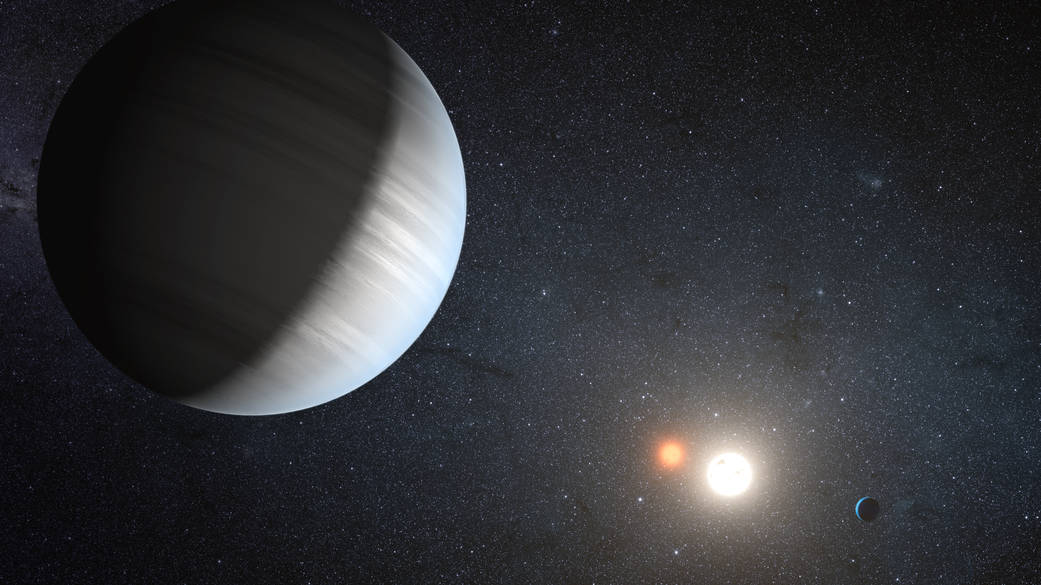
\includegraphics[width=\textwidth]{kepler.jpg}
     \caption{Sharing the Light of Two Suns \cite{kepler}}
\end{center}
   
  \end{figure}
%\end{center}
% -------------    PICTURE ENDS HERE   ---------------

\newpage
\pagenumbering{arabic}
%\doublespacing
% --------------- COVER PAGE ENDS HERE ---------------

% ---------------  QUOTE STARTS HERE   ---------------
\begin{center}
  "If we stay on Earth forever, there will be some eventual extinction event." 
  \end{center}
\begin{flushright}
  -Elon Musk \cite{musk}
\end{flushright}
% ---------------    QUOTE ENDS HERE   ---------------

\begin{abstract}
  This physics Investigation is called "Determining the Goldilocks Zone for 8 stars of different types".
  During this investigation, I will pick 10 random stars of different types: White Dwarfs, Red Giants, Main-Sequence Stars and Red Dwarfs.
  I will research the stars in terms of luminosty, radius and the length of Goldilock Zones, more known as Circumferential Habitable Zones.
  During this research, I will investigate different properties and charasteristics of a star to determine its habitability.
  At the end of the research, we will understand which star types are more preferrable for life.
  For the sake of demonstration, I have written several programs and simulations to support my investigation. 
  \end{abstract}

\newpage

\section{Inroduction}

Soon, our Mother-Star, Sun will make the poles of Earth a tropical paradise and later on destroy all the life on Earth. Approximately in 5.4 billion years, the critical amount of hydrogen in Sun's core will be depleted. In that event, because of lack of hydrogen, Sun will start collapsing under its own weight. The delicate balance between fusion energy and the gravitational pull has fallen.

This catastrophic event forces the core of our Star to contract and therefore, to start fusion of Helium and more heavy elements. This will stop the active contraction of the star but in this event, Sun will burst a colossal amount of energy into outer layers, thus increasing in size so much, that out star will "eat" Mercury and Venus, scientists are not sure about Earth. We can be sure in one fact -  by that time, all the life on Earth will be ceased. Indeed, life will cease to exist way before the Sun's Red Giant phase.

Around in 1.1 billion years, Sun's luminosity will increase by about 10\%. It seems not that much, however, this increase in luminosity will cause a very big shift in Sun's Goldilock zone length. The more active greenhouse effect will take place on Earth, transforming our home planet into a hot, dry and unhabitable planet that Venus is right now.\cite{sun}

As the means of humanity's future survival, we will be forced to leave our planet Earth and find a new planet, new home that maybe can recall our Earth. In order to do that, we should know which planets are habitable and which are not. I will take 8 stars of different types to figure out, what types of stars can host life.

\section{Research question}

My phsyics investgation is aimed at finding the best odds of living near different types of stars, more differentiated by their spectral type. These include: White Dwarfs, Red Giants, Red Dwarfs, and Main-Sequence Stars.\\

\textbf{The research question is}

\textit{What is the relationship between star's spectral type and the conditions of existence of life in the Goldilock Zone}

\section{Hypothesis}

Today, life on Earth is the only known habited planet. We have no information or confirmation about the existence of other life forms and species on other extraterrestial objects. Earth rotates its home star - Sun, which is a typical member of Main-Sequence stars.\\

\textbf{My hypothesis is}

  \textit{The most favorable conditions for life formations are near the members of Main-Sequence stars.}

  \newpage
%  \singlespacing
  \section{Variables list}

\subsection{Dependent variables}
  
  \begin{itemize}

    \item Astronomical distance to a star, $d$ ($pc$)

    \item Absolute Visual Magnutade of a star, $M_V$ ($unit$)
      
    \item Inner Edge of Goldilock Zone of a star, $D_L$ ($AU$) 

      \item Outer Edge of Goldilock Zone of a star, $D_U$ ($AU$)

        \item Bolometric Magnitude, $M_{bol}$ ($unit$)

          \item Apparent Brightness, $b$ ($W m^{-2}$)
          
  \end{itemize}

  \subsection{Controlled variables}

  \begin{itemize}

    \item Apparent Visual Magnutuse of a star, $M$ ($unit$ *from database)

    \item Stefan-Boltzmann constant, $\delta$ ($5.67 \times 10^{-8} W m^{-2} K^{-4}$)

    \item Bolometric Correction, $BC$ ($unit$ *from database)

    \item Parallax to a star, $p$ ($arcsecond$ *from database)

    \item Solar Luminosity, $L_{\odot}$ ($3.828 \times 10^{26}W$)

    \item Astronomical Unit, $AU$ ($150 \times 10^{9}m$)
      
    \end{itemize}


  \section{Database}
  \label{database}
  The HYG Database \cite{hyg} will be used for extraction and parsing of astronomical data. The database contains more than 120,000 stars and it can provide me with the needed data, as the apparent visual magnitudes of stars. 

  \section{Stars}

  Now, we need to choose our 8 stars. For the sake of demonstration and visualization, I wrote a small program in Python \ref{stars} that takes the values from the database \ref{database} and plots Hertzprung-Russel Diagram. Note that instead of luminosity and temperature, values of absolute visual magnitutes and color indexes are used.

  I will take 8 stars of 4 different types, so 2 stars of each type. In the next table, Red Dwarfs, Main-Sequence stars, Red Giants, White Dwarfs are presented, respectively. Table \ref{stars} demonstrates 8 stars that I choosed for research.

  \begin{table}[h]
  \begin{center}
    \begin{tabular}{l l l l}
      \textbf{GlieseID} & \textbf{Star name} & \textbf{Type} & \textbf{Spectra}\\
      551 & Proxima Centauri & Red Dwarf & M5Ve\\
      623 & Gliese 623 & Red Dwarf & M3\\
      482A & 29Gam Vir & Main-Sequence & FOV+...\\
      231 & Alp Men & Main-Sequence & G5V\\
      286 & Pollux & Red Giant & K0IIIvar\\
      841 & HD 208527 & Red Giant & M0\\
      35 & Van Maan & White Dwarf & DG\\
      440 & LP 145-141 & White Dwarf & DC:\\
    \end{tabular}
    \caption{Chosen 8 stars for the investigation.}
    \label{stars}
  \end{center}
    \end{table}


















  
  \singlespacing
  \newpage
  \tiny
  \appendix
  \section{Source code of the Hertzprung-Russel Diagram plotting program}
  \label{hr}
  \begin{lstlisting}
    from tqdm import tqdm
    import matplotlib.pyplot as plt
    import csv
    import math
    import time
    ax = plt.gca()
    ax.set_facecolor('black')
    stars_abs_mag = []
    stars_color_index = []

    #White Dwarfs, Main sequence, Red Giants, Super Giants
    stars_types = [0.0, 0.0, 0.0, 0.0]

    def save_figure(cname, cdpi):
    plt.savefig('{}.png'.format(cname), dpi = cdpi, format = 'png')
    plt.savefig('{}.svg'.format(cname), dpi = cdpi, format = 'svg')

    print(``Extracting stars' data from the database...'')

    with open('HYG-Database/hygdata_v3.csv', 'r') as file:
    cord = csv.reader(file)
    counter = 0
    added_values = 0
    for row in tqdm(cord):
    if not counter == 0 and counter % 25 == 0 or counter == 1:
    # We are skipping first row, as it is text title, not needed
    if not row[16] == '': #If its empty, skip it
    stars_abs_mag.append(float(row[14]))
    stars_color_index.append(float(row[16]))

    if stars_abs_mag[added_values] < -5.0:
    stars_types[3] += 1
    elif stars_abs_mag[added_values] > 10.0 and stars_color_index[added_values] < 1.0:
    stars_types[0] += 1
    elif stars_abs_mag[added_values] < 5.0 and stars_abs_mag[added_values]
    > -5.0 and stars_color_index[added_values] > 0.75:
    stars_types[2] += 1

    added_values+=1
    counter += 1
    file.close()

    plt.scatter(stars_color_index, stars_abs_mag, s = 0.37, c = 'w')

    plt.annotate('Sun', xy = (stars_color_index[0], stars_abs_mag[0]))

    print (``\nOur sun: \n\
    \tAbsolute magnitude : {}\n\
    \tColor index : {}\n''.format(stars_abs_mag[0], stars_color_index[0]))

    stars_types[1] = added_values-stars_types[0]-stars_types[2]-stars_types[3]

    print(``Statistics :\n\
    \t Parsed stars : {} ({}%)\n\
    \t Main Sequence: {} ({}%)\n\
    \t Read Giants  : {} ({}%)\n\
    \t White Dwarfs : {} ({}%)\n\
    \t Super Giants : {} ({}%)\n''.format(added_values,
    round(added_values/added_values*100, 2),
    stars_types[1],
    round(stars_types[1]/added_values*100, 2),
    stars_types[2],
    round(stars_types[2]/added_values*100, 2),
    stars_types[0],
    round(stars_types[0]/added_values*100, 2),
    stars_types[3],
    round(stars_types[3]/added_values*100, 2)
    ))

    plt.ylim([15, -10])
    plt.xlim([-0.5, 2])

    plt.xlabel('Color index')
    plt.ylabel('Absolute magnitude')

    plt.title('Hertzprung-Russel diagram')
    print('Saving the diagrams...')
    save_figure('pics/HRD', 2500)
    print('Done!')


    plt.show()
    \end{lstlisting}

  
% --------------- REFERENCES START HERE ------------------
  \newpage
  \normalsize
\singlespacing
\bibliographystyle{ieeetr}
\bibliography{main}
% --------------- REFERENCES  END  HERE ------------------
  \end{document}
